\documentclass[a4paper]{article}

\usepackage{amsfonts, amsmath, amssymb, amsthm}
\usepackage{graphicx}
\usepackage{fullpage}
\usepackage{float}

\usepackage{tikz}
\usetikzlibrary{calc}

\newtheorem{lemma}{Lemma}
\newtheorem{theorem}{Theorem}
\newtheorem{corollary}{Corollary}
\newtheorem{conjecture}{Conjecture}

\newcommand{\Z}{\mathbb{Z}}
\newcommand{\N}{\mathbb{N}}
\renewcommand{\qedsymbol}{$\blacksquare$}
\newcommand{\abs}[1]{\left| #1 \right|}
\renewcommand{\dim}[1]{\text{dim}\left( #1 \right)}

\setlength{\parindent}{0em}
\setlength{\parskip}{1em}

\begin{document}
	\title{Most Moves Problem in \textit{Lights Out}}
	\author{William Boyles}
	\date{\today}
	\maketitle
	
	\section{Introduction}
	The game \textit{Lights Out}, manufactured by Tiger Electronics, is played on a simple $n \times n$ grid graph $G=(V,E)$ where each vertex consists of a clickable light.
	A move consists of clicking any vertex $v$, which toggles the on/off state of $v$ and its neighbors.
	Starting from an initial configuration of lights, one wins the game by finding a sequence of moves that turns off all the lights.
	Sutner shows that clicking a light twice is equivalent to not clicking it at all \cite{Sutner1989}.
	Thus, we seek a subset of vertices as a solution rather than a sequence.
	One natural question to ask about \textit{Lights Out} is what we call the Most Moves Problem (MMP):
	\begin{quote}
		How many moves does the worst case initial configuration on $G$ require to solve?
	\end{quote}
	Anderson and Feil show that some initial configurations cannot be solved \cite{anderson_feil}.
	Thus, we restrict our attention only to solvable initial configurations.
		
	Eriksson, Eriksson, and Sjöstrand consider arbitrary simple graphs and show that answer to the MMP is a worst-case $\abs{V}$ if and only the number of perfect matchings in $G$ is odd \cite{ERIKSSON2001357}.
	Also focusing on arbitrary simple graphs, Sutner shows that the function $\Phi_G: P(V) \to P(V)$, that maps which vertices are clicked to which vertices turn on is linear with respect to symmetric difference.
	That is, for all $V_1, V_2 \subseteq V$,
	\begin{equation*}
		\Phi_G(V_1 \triangle V_2) = \Phi_G(V_1) \triangle \Phi_G(V_2).
	\end{equation*}
	Further, Sutner shows that $\Phi_G$ is a bijection if and only if the answer to the MMP is the worst case $\abs{V}$.
	Otherwise, the nullity of $G$, $\dim{\ker{\Phi_G}}$ is non-zero and even \cite{Sutner1989}.
	
	We review a technique from Scherphuis to solve the MMP for a $5 \times 5$ grid \cite{jaap}.
	We generalize this approach to give an upper bound the MMP for all grids of size $(6k-1) \times (6k-1)$.
	This upper bound exactly solves the MMP for all such nullity 2 grids.
	We conjecture that this solves the MMP for all nullity 2 grids.
	
	\section{Parity Covers}
	For any vertex $v \in V$, let $N(v)$, the neighborhood of $v$ be all vertices that are affected when we click $v$.
	That is,
	\begin{equation*}
		N(v) = \{u \in V \mid u=v \text{ or } (u,v) \in E\}.
	\end{equation*}
	If we have $V' \subseteq V$ such that for all $v \in V$, $\abs{V' \cap N(v)}$ is even, then we say $V'$ is an even parity cover of $G$.
	We can analogously define odd parity covers.
	Sutner showed that every graph has an odd parity cover but, not every graph has an even parity cover other than the trivial $V' = \emptyset$ \cite{Sutner1989}.
	
	\begin{lemma}\label{empty-is-even}
		Let $V' \subseteq V$.
		Then $V'$ even parity cover of $G$ if and only if $\Phi_G(V') = \emptyset$.
	\end{lemma}
	\begin{proof}
		We know from Sutner that the state of vertex $v$ depends only on how often (even or odd) elements of $N(v)$ have been clicked \cite{Sutner1989}.
		So, for $V' \subseteq V$, $\Phi_G(V') = \emptyset$ is equivalent to every vertex containing an even number of elements from $V'$ in its neighborhood.
		This is exactly the definition of $V'$ being an even parity cover.
	\end{proof}
	
	\begin{lemma}
		Let $V'$ be an even parity cover of $G$, and let $V_1 \subseteq V$.
		If $V_1$ is the solution to some initial configuration, then so is $V_1 \triangle V'$.
	\end{lemma}
	\begin{proof}
		We know that $\Phi_G$ is linear with respect to symmetric difference.
		So,
		\begin{align*}
			\Phi_G(V_1) &= \Phi_G(V_1) \triangle \emptyset \\
			&= \Phi_G(V_1) \triangle \Phi_G(V') \\
			&= \Phi_G(V_1 \triangle V'),
		\end{align*}
		as desired.
	\end{proof}

	\begin{lemma}
		Let $V_1$ and $V_2$ be solutions to the same initial configuration.
		Then $V_1 \triangle V_2$ is an even parity cover of $G$.
	\end{lemma}
	\begin{proof}
		Since $V_1$ and $V_2$ are solutions to the same initial configuration, $\Phi_G(V_1) = \Phi_G(V_2)$.
		So,
		\begin{align*}
			\Phi_G(V_1 \triangle V_2) &= \Phi_G(V_1) \triangle \Phi_G(V_2) \\
			&= \Phi_G(V_1) \triangle \Phi_G(V_1) \\
			&= \emptyset.
		\end{align*}
		Thus, by Lemma \ref{empty-is-even}, $V_1 \triangle V_2$ is an even parity cover of $G$.
	\end{proof}

	These lemmas show that to find the solution to a given initial configuration that uses the fewest moves, we simply need to find any solution to the initial configuration.
	We can then apply every even parity cover to generate all equivalent solutions, one of which will be the smallest.
		
	\section{MMP for $5 \times 5$ Grid}
	The $5 \times 5$ grid is smallest with $\dim{\ker{\Phi_G}} = 2$.
	Since we will apply nearly the same techniques in the next section, we will restate Scherphuis's proof of solving the MMP for a $5 \times 5$ grid in our own notation.
	\begin{theorem}[Scherphuis]\label{min-moves-problem-5x5}
		The answer to the Min Moves Problem for a $5 \times 5$ grid graph is 15.
	\end{theorem}
	\begin{proof}
		Since $\dim{\ker{\Phi_G}} = 2$, there are $2^2 = 4$ even parity covers of a $5 \times 5$ grid.
		One of these even parity covers is the trival empty set.
		Below are the three non-trivial even parity covers.
		A black square means the corresponding vertex is an element of the even parity cover.
		
		\begin{figure}[H]
			\centering
			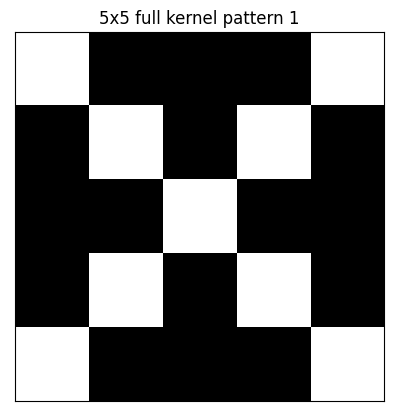
\includegraphics[width=0.32\textwidth]{../../code/serialization/kernels/5x5/full/5x5_kernel_full_1.png}
			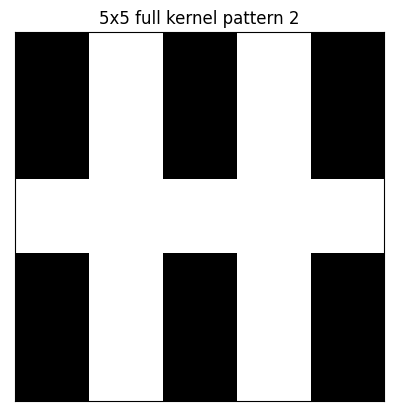
\includegraphics[width=0.32\textwidth]{../../code/serialization/kernels/5x5/full/5x5_kernel_full_2.png}
			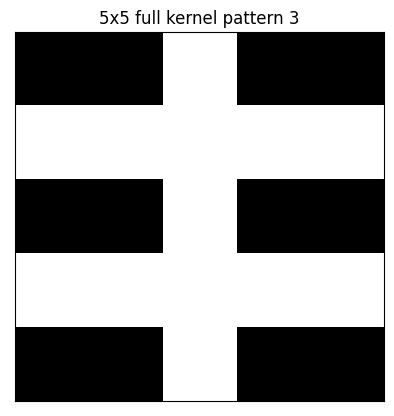
\includegraphics[width=0.32\textwidth]{../../code/serialization/kernels/5x5/full/5x5_kernel_full_3.png}
			\caption{Non-trivial elements of $\ker{\Phi_G}$ for $G$ a $5 \times 5$ grid}
		\end{figure}
	
		As shown below, partition the vertices of the $5 \times 5$ grid to one of four regions based on which even parity covers contain them.
		
		\begin{figure}[H]
			\centering
			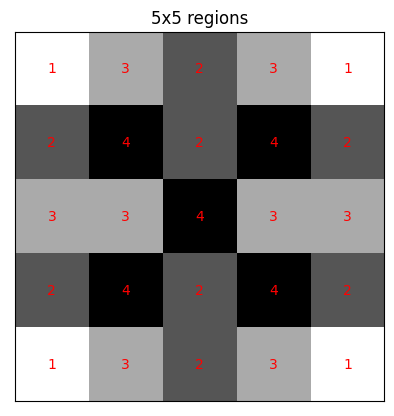
\includegraphics[width=0.49\textwidth]{../../code/serialization/regions/5x5_regions.png}
			\caption{The four regions of a $5 \times 5$ grid}
		\end{figure}
	
		Region 1 is the intersection of covers 2 and 3;
		region 2 is the intersection of  covers 1 and 2;
		region 3 is the intersection of covers 1 and 3;
		region 4 is the intersection of all the complements.
		
		Let $Y \subseteq V$ be a worst case initial configuration.
		Let $X \subseteq V$ be a solution to $Y$ that uses the fewest moves among all solutions to $Y$.
		Let $R_i$ be the number of vertices in $X$ also contained in region $i$.
		Then the solution uses $\abs{X} = R_1 + R_2 + R_3 + R_4$ moves.
		
		If we take the symmetric difference of $X$ and even parity cover 1, we obtain an equivalent solution that uses $R_1 + (8 - R_2) + (8 - R_3) + R_4$ moves.
		Since we assumed $X$ was a minimal solution,
		\begin{equation*}
			R_1 + R_2 + R_3 + R_4 \leq R_1 + (8 - R_2) + (8 - R_3) + R_4.
		\end{equation*}
		Rearranging,
		\begin{equation}\label{5x5_constr1}
			R_2 + R_3 \leq 8.
		\end{equation}
	
		If we take the symmetric difference of $X$ and even parity cover 2, we obtain an equivalent solution that uses $(4 - R_1) + (8 - R_2) + R_3 + R_4$ moves.
		Since we assumed $X$ was a minimal solution,
		\begin{equation*}
			R_1 + R_2 + R_3 + R_4 \leq (4 - R_1) + (8 - R_2) + R_3 + R_4.
		\end{equation*}
		Rearranging,
		\begin{equation}\label{5x5_constr2}
			R_1 + R_2 \leq 6.
		\end{equation}
	
		If we take the symmetric difference of $X$ and even parity cover 3, we obtain an equivalent solution that uses $(4 - R_1) + R_2 + (8 - R_3) + R_4$ moves.
		Since we assumed $X$ was already a minimal solution,
		\begin{equation*}
			R_1 + R_2 + R_3 + R_4 \leq (4 - R_1) + R_2 + (8 - R_3) + R_4.
		\end{equation*}
		Rearranging,
		\begin{equation}\label{5x5_constr3}
			R_1 + R_3 \leq 6.
		\end{equation}
	
		Since we have applied all even parity covers, we can be sure we considered all solutions to $Y$.
		None of \eqref{5x5_constr1}, \eqref{5x5_constr2}, or \eqref{5x5_constr3} involve $R_4$.
		Thus, $R_4$ is not constrained beyond the fact that region 4 contains five vertices.
		Since we assumed $Y$ was a worst case initial configuration, $R_4 = 5$.
	
		Combining \eqref{5x5_constr1}, \eqref{5x5_constr2}, and \eqref{5x5_constr3} into matrix form,
		\begin{equation}\label{5x5_ilp}
			\begin{bmatrix}
				0 & 1 & 1 \\
				1 & 1 & 0 \\
				1 & 0 & 1
			\end{bmatrix}
			\begin{bmatrix}
				R_1 \\
				R_2 \\
				R_3
			\end{bmatrix}
			\leq
			\begin{bmatrix}
				8 \\
				6 \\
				6
			\end{bmatrix}.
		\end{equation}
		Thus, because we assumed $Y$ was a worst case initial configuration, $R_4 = 5$., we need to solve this integer linear program (ILP), maximizing the $L^1$-norm $R_1 + R_2 + R_3$.
		Since all entries in the constraint matrix of \eqref{5x5_ilp} are non-negative, finding an integer solution where the constraints are tight (i.e. replace the $\leq$ in \eqref{5x5_ilp} with $=$) would be the optimal solution to the ILP.
		
		Assuming the constraints are tight and performing row reduction, we find that
		\begin{equation*}
			\begin{bmatrix}
				R_1 \\
				R_2 \\
				R_3
			\end{bmatrix}
			=
			\begin{bmatrix}
				2 \\
				4 \\
				4
			\end{bmatrix}
		\end{equation*}
		is the optimal solution to the ILP.
		So, the answer to the Min Moves Problem for a $5 \times 5$ grid is $\abs{X} = R_1 + R_2 + R_3 + R_4 = 2 + 4 + 4 + 5 = 15$.
	\end{proof}

	\section{Inequality for Larger Grids}
	If we have an even parity cover for a smaller grid, we can construct an even parity cover for a larger grid.
	
	\begin{theorem}\label{tiling-quiet-patterns}
		Let $d(n) = \dim{\ker{\Phi_G}}$ for $G$ an $n \times n$ grid.
		Then for all $n,k \in \N$,
		\begin{equation*}
			d(nk - 1) \geq d(n-1).
		\end{equation*}
	\end{theorem}
	\begin{proof}
		Let $n,k \in \N$.
		Since $nk - 1 = k(n-1) + (k-1)$, an $(nk-1) \times (nk-1)$ grid consists of a $k \times k$ grid of $(n-1) \times (n-1)$ grids, each separated by a horizontal or vertical strip of height or width 1.
	
		Let $Q \subseteq V$ be an even parity cover for an $(n-1) \times (n-1)$ grid.
		Let $R$ be $Q$ tiled $k$ times horizontally and vertically onto an $(nk-1) \times (nk-1)$ grid, where each tile is a horizontal/vertical reflection of its horizontal/vertical neighboring tiles, as shown below.
		
		\begin{figure}[H]
			\centering
% Code the generate figure w/o Q's
%			\begin{tikzpicture}[scale=0.33]
%				\edef\M{3} % Width of each tile
%				\edef\K{5} % Number of tiles in each direction
%				\pgfmathparse{(\M+1)*\K - 1} % Size of large grid
%				\edef\N{\pgfmathresult}
%				
%				\draw[black,thin] (0,0) grid (\N,\N);
%				
%				\foreach \i in {1,2,...,\K}{
%					\foreach \j in {1,2,...,\K}{
%						\pgfmathparse{(\i - 1) * (\M + 1)}
%						\edef\X{\pgfmathresult}
%						\pgfmathparse{(\j - 1) * (\M + 1)}
%						\edef\Y{\pgfmathresult}
%						
%						\draw[fill,gray,opacity=0.707] (\X, \Y) rectangle (\X + \M, \Y + \M);
%						%\node at (\X + \M/2, \Y + \M/2) {$Q$};
%					}
%				}
%			\end{tikzpicture}
			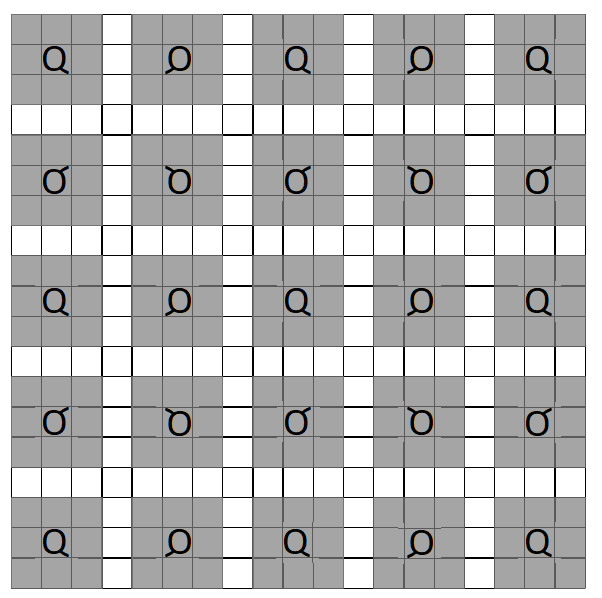
\includegraphics[width=0.5\textwidth]{tiling_q.png}
			\caption{Pattern $Q$ tiled 5 times.}	
		\end{figure}
	
		Consider any vertex $v$ in the $(nk-1) \times (nk-1)$ grid.
		If $v$ is in one of the areas containing a reflection of $Q$, then $N(v) \cap R$ is even because $Q$ is an even parity cover.
		Otherwise, $v$ is in one of the borders between reflections of $Q$.
		So, $N(v)$ contains either zero or two vertices that are in a reflection of $Q$.
		If $N(v)$ contains zero such vertices, then $\abs{N(v) \cap R} = 0$, which is even.
		If $N(v)$ contains two such vertices, then these vertices are either both in $R$ or neither are in $R$.
		Thus, $\abs{N(v) \cap R}$ is even.
		So, $R$ is an even parity cover.
		
		So, each even parity cover of an $(n-1) \times (n-1)$ grid allows us to generate a unique even parity cover for an $(nk-1) \times (nk-1)$ grid.
		Since these even parity covers are independent on a $(n-1) \times (n-1)$ grid, they are also independent on the larger $(nk-1) \times (nk-1)$ grid.
		Thus,
		\begin{equation*}
			d(nk-1) \geq d(n-1),
		\end{equation*}
		as desired.
	\end{proof}

	\section{Establishing an Upper Bound}
	Applying Theorem \ref{tiling-quiet-patterns} for $n=6$, we get that for all $k \in \N$,
	\begin{equation*}
		d(6k - 1) \geq d(5) = 2.
	\end{equation*}
	So, tilings of even parity covers from a $5 \times 5$ grid are also even parity covers of $(6k-1) \times (6k-1)$ grids.
	For example, notice how the $17 \times 17$ even parity covers are simply the $5 \times 5$ even parity covers tiled $k=3$ times.
	
	\begin{figure}[H]
		\centering
		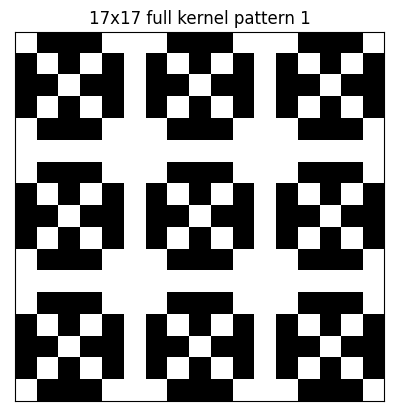
\includegraphics[width=0.32\textwidth]{../../code/serialization/kernels/17x17/full/17x17_kernel_full_1.png}
		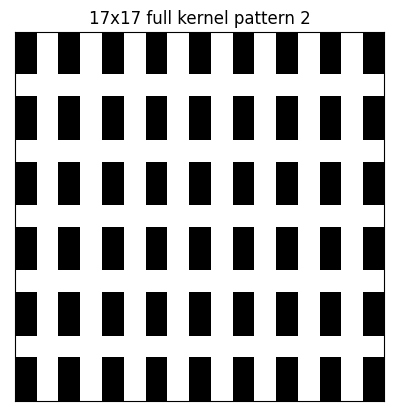
\includegraphics[width=0.32\textwidth]{../../code/serialization/kernels/17x17/full/17x17_kernel_full_2.png}
		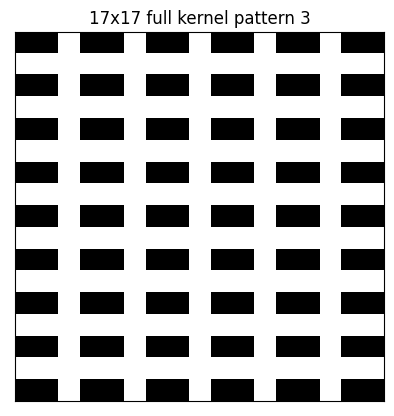
\includegraphics[width=0.32\textwidth]{../../code/serialization/kernels/17x17/full/17x17_kernel_full_3.png}
		\caption{Non-trivial elements of $\ker{\Phi}$ for $G$ a $17 \times 17$ grid}
	\end{figure}
	
	Thus, we can apply the same proof technique as in Theorem \ref{min-moves-problem-5x5} to find an upper bound for the Min Moves Problem for such grid sizes.
	We'll also know that if $d(6k - 1) = 2$, then we have considered all equivalent solutions, meaning this upper bound is exact, and we have solved the Min Moves Problem.
	
	\begin{theorem}\label{min-moves-problem-6k-1x6k-1}
		Let $k \in \N$.
		Then the answer to the MMP for a $(6k - 1) \times (6k - 1)$ grid is at most $26k^2 - 12k + 1$.
		This bound is exactly the answer to the MMP when $d(6k-1)=2$.
	\end{theorem}
	\begin{proof}
		Let $k \in \N$.
		Applying Theorem \ref{tiling-quiet-patterns} with $n=6$, the even parity covers of the $5 \times 5$ grid will tile a $(6k - 1) \times (6k - 1)$ grid.
		We can partition the vertices of the grid into four regions based on which of these even parity covers they are a part of.
		Using the same numbering for even parity covers as in Theorem \ref{min-moves-problem-5x5}, region 1 is the intersection of even parity covers 2 and 3;
		region 2 is the intersection of even parity covers 1 and 2;
		region 3 is the intersection of even parity covers 1 and 3;
		region 4 is the intersection of the complements.
		Region 1 contains $4k^2$ vertices, regions 2 and 3 contain $8k^2$ vertices, and region 4 contains the remaining $16k^2 - 12k + 1$ vertices.
		
		Let $Y \subseteq V$ be a worst case initial configuration/
		Let $X \subseteq V$ be a solution to $Y$ that uses the fewest moves among all solutions to $Y$.
		Let $R_i$ be the number of vertices in $X$ also contained in region $i$.
		Then the solution uses $\abs{X} = R_1 + R_2 + R_3 + R_4$ moves.
		
		Applying the three even parity covers and deriving the constraints like we did in proving Theorem \ref{min-moves-problem-5x5}, we find that $R_4$ is unconstrained and can thus be set to $16k^2 - 12k + 1$, while $R_1$, $R_2$, and $R_3$ are constrained by the following ILP:
		\begin{equation}
			\begin{bmatrix}
				0 & 1 & 1 \\
				1 & 1 & 0 \\
				1 & 0 & 1 
			\end{bmatrix}
			\begin{bmatrix}
				R_1 \\
				R_2 \\
				R_3
			\end{bmatrix}
			\leq
			\begin{bmatrix}
				8 \\
				6 \\
				6
			\end{bmatrix}k^2.
		\end{equation}
		This is the exact same set of constraints as in Theorem \ref{min-moves-problem-5x5}, just with a factor of $k^2$.
		Thus,
		\begin{equation*}
			\begin{bmatrix}
				R_1 \\
				R_2 \\
				R_3
			\end{bmatrix}
			=
			\begin{bmatrix}
				2 \\
				4 \\
				4
			\end{bmatrix}k^2.
		\end{equation*}
		is the solution to the ILP.
		Thus, $\abs{X} = R_1 + R_2 + R_3 + R_4 = 2k^2 + 4k^2 +  4k^2 + 16k^2 - 12k + 1 = 26k^2 - 12k + 1$.
		
		If $\dim{\ker{\Phi}} > 2$ there will be more even parity covers that would create more restrictive constraints.
		However, if $\dim{\ker{\Phi}} = 2$, we have considered all even parity covers and have solved the MMP.
	\end{proof}

	The $5 \times 5$, $17 \times 17$, $41 \times 41$, $53 \times 53$, $77 \times 77$, grids are those of size $(6k-1) \times (6k-1)$ less than 100 with nullity 2.
	Thus, we find that the answers to the MMP for these grids are 15, 199, 1191, 1999, and 4239 respectively.
	
	\section{Conjectures}
	\begin{conjecture}\label{infinite-nullity-2}
		There are infinitely many $n$ such that $d(n) = 2$.
	\end{conjecture}
	We already know that the version of this conjecture with $d(n)=0$ is true.
	Sutner mentions that the nullity of all $(2^k - 1) \times (2^k - 1)$ grids for $k \in \N$ is 0 \cite{Sutner1989}.
	Theorem \ref{tiling-quiet-patterns} tells us that there are infinitely many $n$ with $d(n) \geq 2$.
	By computer search we found that there are 497 such $n$ for $n \leq 10000$.
	
	\begin{conjecture}\label{all-nullity2-conj}
		If an $n \times n$ grid has nullity 2, then $n \equiv -1 \mod 6$.
	\end{conjecture}
	That is, the even parity covers of all nullity 2 grids are tilings of the $5 \times 5$ even parity covers.
	If true, this would mean that we have solved the MMP for all nullity 2 grids.
	Applying Theorem \ref{tiling-quiet-patterns} in a sieve approach to eliminate grids we know have nullity greater than 2, we performed a computer search and found no counterexamples for $n \leq 10000$.
	
	\section{Future Work}
	We'd like future work to focus on resolving the above conjectures and solving the MMP on grids with nullities greater than 2.
	For any sized grid (in fact, any graph), we can apply the same technique as in theorems \ref{min-moves-problem-5x5} and \ref{min-moves-problem-6k-1x6k-1} of finding the answer to the Min Moves Problem as the solution to an ILP.
	However, it seems we cannot apply the same technique of trying to solve the ILP with all constraints tight for larger nullities.
	
	We'd also like future work to focus more on understanding the relationships between the nullities of different sized grids.
	Theorem \ref{tiling-quiet-patterns} is a good start to this, but there seem to be many other patterns to discover.
	For example, Knuth shows that if an even parity cover of an $n \times n$ grid is perfect -- no row or column contains no elements from the cover -- then we can construct a perfect even parity cover for a $(2n+1) \times (2n+1)$ grid \cite{Knuth_AOCP4A}.
	All the even parity covers constructed in Theorem \ref{tiling-quiet-patterns} are not perfect.
	Also, Sutner conjectures that $d(2n+1) = 2d(n) + \delta_n$, where $\delta_n \in \{0,2\}$, and $\delta_{2n+1} = \delta_n$ \cite{Sutner1989}.
	
	\newpage
	\bibliography{refs.bib}
	\bibliographystyle{plain}
\end{document}